\section{Code Architecture and Structure}
\begin{figure}[!htb]
    \centering
    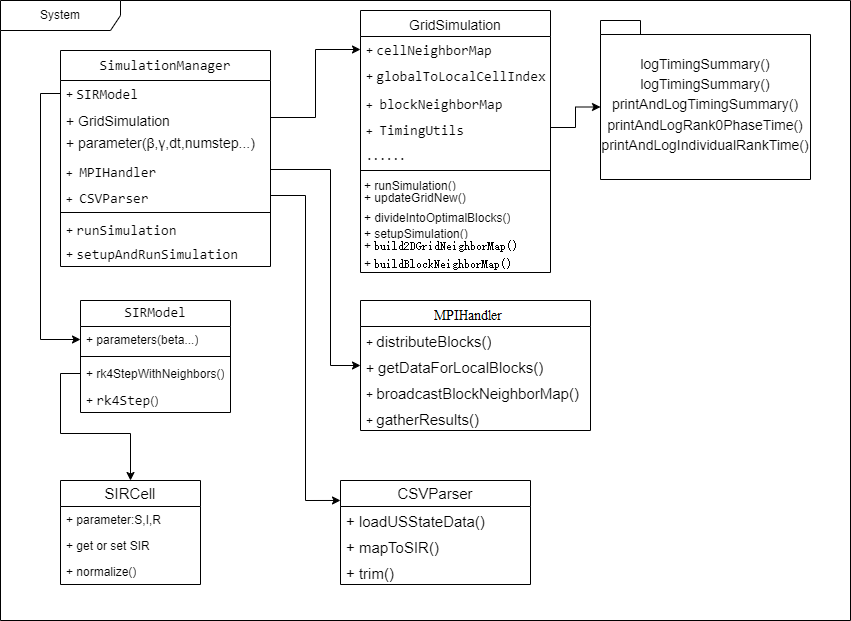
\includegraphics[width=12cm]{Images/pic0.png}
\end{figure}


\subsection{CSVParser Class}
The \texttt{CSVParser} class is responsible for reading and preprocessing real-world COVID-19 data from CSV files. It extracts relevant fields such as population, confirmed, recovered, and active cases, and converts them into normalized SIR values. The parsed data is returned as \texttt{SIRCell} instances, ensuring that each cell satisfies \( S + I + R = 1 \) through internal normalization.


\subsection{SIRCell Class}
This class encapsulates the state variables of each simulation cell: susceptible (S), infected (I), and recovered (R). It provides getter and setter methods with bounds checking to ensure physical validity.  
After each update, we apply a \texttt{normalize()} method that rescales the values so that \( S + I + R = 1 \).  

This normalization is not part of the classical SIR model itself, but a design choice introduced in our implementation to mitigate numerical drift and maintain probabilistic consistency.


\subsection{SIRModel Class}
The \texttt{SIRModel} class defines the evolution equations and implements two versions of the Runge-Kutta 4th-order integration: one for isolated cells, and one that incorporates neighbor influence (\texttt{rk4StepWithNeighbors}). It holds model parameters such as \( \beta \), \( \gamma \), timestep size, and total number of steps.

\subsection{GridSimulation Class}
This class is responsible for managing the entire simulation grid, including the local cells, global-to-local ID mappings, and ghost regions. It handles the step-by-step evolution of the system, sets up the neighbor relations, and maintains grid partitioning and block ownership across ranks.

\subsection{TimingUtils}
The \texttt{TimingUtils} provides utility functions for logging and analyzing the runtime performance of the simulation. It records the execution time of each phase (e.g., initialization, communication, computation) across all MPI ranks. The class supports generating both global and rank-specific timing summaries, including minimum, maximum, and average statistics. This data helps identify bottlenecks and evaluate the scalability of the simulation framework.

\subsection{MPIHandler and SimulationManager Classes}
The \texttt{MPIHandler} class abstracts all MPI-related communication, including distributing grid blocks, exchanging ghost cells, and gathering final results. The \texttt{SimulationManager} class coordinates the entire simulation workflow: loading data, initializing components, running the main loop, and storing output.

\subsection{Design Principles and Code Organization}
The code is structured with modularity and scalability in mind. Core logic is separated from communication routines, and all timing-related functionality is encapsulated in a utility module. The design ensures clear responsibility separation and allows easy testing or extension (e.g., for other ODE models or input formats).
